\documentclass[spanish,a4paper,11pt,twoside]{report}

%%%%%%%%%%%%%%%%%%%%%%%%%%%%%%%%%%%%%%%%%%%%%%%%%%%%%%%%%%%%%%%%%%%%%%%%%%%%%%%
\usepackage{graphicx}
\usepackage[dvips]{epsfig}
\usepackage[latin1]{inputenc}
\usepackage[spanish]{babel}
\usepackage{alltt}
\usepackage{algorithm}
\usepackage{algorithmic}
\usepackage{multirow}

\usepackage{haskelllogo}

%%%%%%%%%%%%%%%%%%%%%%%%%%%%%%%%%%%%%%%%%%%%%%%%%%%%%%%%%%%%%%%%%%%%%%%%%%%%%%%

\newcommand{\SONY}{{\sc Sony}}
\newcommand{\MICROSOFT}{{\sc Microsoft}}
\newcommand{\GCC}{\textsf{\textsc{G}CC}}
\newcommand{\INTEL}{\textsf{\textsc{I}ntel}}

%%% Traducimos el pseudo�digo
\renewcommand{\algorithmicwhile}{\textbf{mientras}}
\renewcommand{\algorithmicend}{\textbf{fin}}
\renewcommand{\algorithmicdo}{\textbf{hacer}}
\renewcommand{\algorithmicif}{\textbf{si}}
\renewcommand{\algorithmicthen}{\textbf{entonces}}
\renewcommand{\algorithmicrepeat}{\textbf{repetir}}
\renewcommand{\algorithmicuntil}{\textbf{hasta que}}
\renewcommand{\algorithmicelse}{\textbf{en otro caso}}
\renewcommand{\algorithmicfor}{\textbf{para}}

%\newcommand{\RETURN}{\textbf{retornar} }
\newcommand{\RET}{\STATE \textbf{retornar} }
\newcommand{\TO}{\textbf{hasta} }
\newcommand{\AND}{\textbf{y} }
\newcommand{\OR}{\textbf{o} }

%%%%%%%%%%%%%%%%% Creamos un entorno para listar c�digo fuente %%%%%%%%%%%%%%%
\newenvironment{sourcecode}
{\begin{list}{}{\setlength{\leftmargin}{1em}}\item\scriptsize\bfseries}
{\end{list}}

\newenvironment{littlesourcecode}
{\begin{list}{}{\setlength{\leftmargin}{1em}}\item\tiny\bfseries}
{\end{list}}

\newenvironment{summary}
{\par\noindent\begin{center}\textbf{Abstract}\end{center}\begin{itshape}\par\noindent}
{\end{itshape}}

\newenvironment{keywords}
{\begin{list}{}{\setlength{\leftmargin}{1em}}\item[\hskip\labelsep \bfseries Keywords:]}
{\end{list}}

\newenvironment{palabrasClave}
{\begin{list}{}{\setlength{\leftmargin}{1em}}\item[\hskip\labelsep \bfseries Palabras clave:]}
{\end{list}}


%%%%%%%%%%%%%%%%%%%%%%%%%%%%%%%%%%%%%%%%%%%%%%%%%%%%%%%%%%%%%%%%%%%%%%%%%%%%%%%
% Format
%%%%%%%%%%%%%%%%%%%%%%%%%%%%%%%%%%%%%%%%%%%%%%%%%%%%%%%%%%%%%%%%%%%%%%%%%%%%%%%

%%\topmargin -4 mm
%\topmargin -21 mm
%\headheight 10 mm
%\headsep 10 mm

%\textheight 229 mm
%\textheight 246 mm

%\oddsidemargin -5.4 mm
%\evensidemargin -5.4 mm
\oddsidemargin 5 mm
\evensidemargin 5 mm

%\oddsidemargin -3 mm
%\evensidemargin -3 mm

%\textwidth 17 cm
\textwidth 15 cm
%\columnsep 10 mm

\input{amssym.def}

%%%%%%%%%%%%%%%%%%%%%%%%%%%%%%%%%%%%%%%%%%%%%%%%%%%%%%%%%%%%%%%%%%%%%%%%%%%%%%%

\begin{document}

%%%%%%%%%%%%%%%%%%%%%%%%%%%%%%%%%%%%%%%%%%%%%%%%%%%%%%%%%%%%%%%%%%%%%%%%%%%%%%%
% First Page 
%%%%%%%%%%%%%%%%%%%%%%%%%%%%%%%%%%%%%%%%%%%%%%%%%%%%%%%%%%%%%%%%%%%%%%%%%%%%%%%

\pagestyle{empty}
\thispagestyle{empty}


\newcommand{\HRule}{\rule{\linewidth}{1mm}}
\setlength{\parindent}{0mm}
\setlength{\parskip}{0mm}
\vspace*{\stretch{1}}

\begin{center}
  
\includegraphics[width=0.2\textwidth]{images/logotipo-secundario-ULL}\\[0.25cm]
\end{center}

\HRule

\begin{minipage}{.25\linewidth}
  \begin{flushleft}
    \noindent
    \haskelllogo[seventies] %%,lambdainfront
  \end{flushleft}
\end{minipage}
%%\hfill
\begin{minipage}{0.75\linewidth}
  \begin{flushright}
    {\Huge Construcci�n de un Compilador} \\[2.5mm] 
    {\Huge y un Int�rprete de Scheme Usando Haskell} \\[2.5mm]
    {\Large \textit{Building a Compiler and Interpreter for Scheme Using Haskell}} \\[5mm]
    {\Large Francisco Nebrera Perdomo} \\[5mm]
    Dpto. de Ingenier�a Inform�tica y de Sistemas \\[5mm]
    Escuela T\'ecnica Superior de Ingenier\'{\i}a Inform\'atica \\[5mm]
    Trabajo de Fin de Grado \\
  \end{flushright}
\end{minipage}

\HRule
\vspace*{\stretch{2}}
\begin{center}
  \Large La Laguna, \today 
\end{center}

\setlength{\parindent}{5mm}

%%%%%%%%%%%%%%%%%%%%%%%%%%%%%%%%%%%%%%%%%%%%%%%%%%%%%%%%%%%%%%%%%%%%%%%%%%%%%%%
% Signature page (add the official stamp)
%%%%%%%%%%%%%%%%%%%%%%%%%%%%%%%%%%%%%%%%%%%%%%%%%%%%%%%%%%%%%%%%%%%%%%%%%%%%%%%
%\newpage
\cleardoublepage
\thispagestyle{empty}

D. {\bf Casiano Rodr�guez Le�n}, con N.I.F. 12.345.678-X 
profesor
Titular de Universidad 
adscrito al Departamento 
de Estad�stica IO y Computaci�n 
de la Universidad de La Laguna

\bigskip
\bigskip
\bigskip
\bigskip
\bigskip
{\bf C E R T I F I C A}

\bigskip
\bigskip
\bigskip
Que la presente memoria titulada:

\bigskip
``{\it Construcci�n de un Compilador y un Int�rprete de Scheme Usando Haskell.}''

\bigskip
\bigskip
\bigskip

\noindent ha sido realizada bajo su direcci�n por D. {\bf Francisco Nebrera Perdomo}, con N.I.F. 79064507-Y.

\bigskip
\bigskip

Y para que as� conste, en cumplimiento de la legislaci�n vigente y a los efectos oportunos firman la presente en La Laguna a \today 

\cleardoublepage
%%%%%%%%%%%%%%%%%%%%%%%%%%%%%%%%%%%%%%%%%%%%%%%%%%%%%%%%%%%%%%%%%%%%%%%%%%%%%%%
\thispagestyle{empty}

{ \flushright

\begin{LARGE}
Agradecimientos
\end{LARGE}

\hspace{3mm}

\begin{large}


\hspace{3mm}
Casiano Rodr�guez Le�n

\hspace{3mm}
Jorge Riera Ledesma

\hspace{3mm}
Luz Marina Moreno de Antonio

\hspace{3mm}
Francisco de Sande Gonz�lez

\hspace{3mm}
Francisco Carmelo Almeida Rodr�guez

\hspace{3mm}
Blas C. Ruiz

\hspace{3mm}
F. Guti�rrez

\hspace{3mm}
P. Guerrero

\hspace{3mm}
E. Gallardo

\hspace{3mm}
Daniel D�az Casanueva


\end{large}

}

%%%%%%%%%%%%%%%%%%%%%%%%%%%%%%%%%%%%%%%%%%%%%%%%%%%%%%%%%%%%%%%%%%%%%%%%%%%%%%%
\cleardoublepage
\begin{abstract}
{\em 

El objetivo de este trabajo ha sido .... 
%
bla, bla, bla
%
bla, bla, bla
%
bla, bla, bla

}

\begin{palabrasClave}
Palabra reservada1, Palabra reservada2, ...
\end{palabrasClave}

\end{abstract}
%%%%%%%%%%%%%%%%%%%%%%%%%%%%%%%%%%%%%%%%%%%%%%%%%%%%%%%%%%%%%%%%%%%%%%%%%%%%%%%

%%%%%%%%%%%%%%%%%%%%%%%%%%%%%%%%%%%%%%%%%%%%%%%%%%%%%%%%%%%%%%%%%%%%%%%%%%%%%%%
\cleardoublepage
\begin{summary}
{\em 

Here should be the abstract in a foreing language...

}

\begin{keywords}
Keyword1, Keyword2, Keyword2, ...
\end{keywords}

\end{summary}
%%%%%%%%%%%%%%%%%%%%%%%%%%%%%%%%%%%%%%%%%%%%%%%%%%%%%%%%%%%%%%%%%%%%%%%%%%%%%%%

%%%%%%%%%%%%%%%%%%%%%%%%%%%%%%%%%%%%%%%%%%%%%%%%%%%%%%%%%%%%%%%%%%%%%%%%%%%%%%%
\newpage{\pagestyle{empty}\cleardoublepage}
\thispagestyle{empty}

%%%%%%%%%%%%%%%%%%%%%%%%%%%%%%%%%%%%%%%%%%%%%%%%%%%%%%%%%%%%%%%%%%%%%%%%%%%%%%%


\pagestyle{myheadings} %my head defined by markboth or markright
% No funciona bien \markboth sin "twoside" en \documentclass, pero al
% ponerlo se dan un mont�n de errores de underfull \vbox, con lo que no se
% ha puesto.
\markboth{Francisco Nebrera Perdomo}{Compilador e int�rprete usando lenguajes funcionales}

%%%%%%%%%%%%%%%%%%%%%%%%%%%%%%%%%%%%%%%%%%%%%%%%%%%%%%%%%%%%%%%%%%%%%%%%%%%%%%%
%Numeracion en romanos
\renewcommand{\thepage}{\roman{page}}
\setcounter{page}{1}

%%%%%%%%%%%%%%%%%%%%%%%%%%%%%%%%%%%%%%%%%%%%%%%%%%%%%%%%%%%%%%%%%%%%%%%%%%%%%%%

\tableofcontents

%%%%%%%%%%%%%%%%%%%%%%%%%%%%%%%%%%%%%%%%%%%%%%%%%%%%%%%%%%%%%%%%%%%%%%%%%%%%%%%
\newpage{\pagestyle{empty}\cleardoublepage}

\listoffigures

%%%%%%%%%%%%%%%%%%%%%%%%%%%%%%%%%%%%%%%%%%%%%%%%%%%%%%%%%%%%%%%%%%%%%%%%%%%%%%%
\newpage{\pagestyle{empty}\cleardoublepage}

\listoftables

%%%%%%%%%%%%%%%%%%%%%%%%%%%%%%%%%%%%%%%%%%%%%%%%%%%%%%%%%%%%%%%%%%%%%%%%%%%%%%%
\newpage{\pagestyle{empty}\cleardoublepage}

%%%%%%%%%%%%%%%%%%%%%%%%%%%%%%%%%%%%%%%%%%%%%%%%%%%%%%%%%%%%%%%%%%%%%%%%%%%%%%%
%Numeracion a partir del capitulo I
\renewcommand{\thepage}{\arabic{page}}
\setcounter{page}{1}


\chapter{Introducci�n}
\label{chapter:intro}

%%%%%%%%%%%%%%%%%%%%%%%%%%%%%%%%%%%%%%%%%%%%%%%%%%%%%%%%%%%%%%%%%%%%%%%%%%%%%
% Chapter 1: Introducci�n 
%%%%%%%%%%%%%%%%%%%%%%%%%%%%%%%%%%%%%%%%%%%%%%%%%%%%%%%%%%%%%%%%%%%%%%%%%%%%%%%

%---------------------------------------------------------------------------------
Todo empez� con un hilo en el foro de internet forocoches.com (\url{https://www.forocoches.com}), en �l hablaban de que la programaci�n funcional iba a tener cada d�a m�s relevancia porque cuenta con ventajas de 
las cuales la imperativa carece.\\

A ra�z de ello, me interes� por este paradigma y empec� a (e incluso termin� de) leer numerosos 
libros sobre el lenguaje y la programaci�n funcional en general, y a crear peque�os programas en 
Haskell. Haskell es muy interesante debido a que es el lenguaje con mayor nivel de 
abstracci�n en el que he programado hasta hoy.\\

Haskell es id�neo para crear lenguajes de dominio espec�fico. En otras palabras, antes de 
escribir un compilador se captura el lenguaje a compilar (el lenguaje fuente) en un 
tipo. Las expresiones de ese tipo representar�n t�rminos en el lenguaje fuente y normalmente son 
bastante similares al mismo, a pesar de ser, realmente, tipos de Haskell.\\

Luego se representa el lenguaje objetivo como otro tipo m�s. Finalmente, el compilador es 
realmente una funci�n del tipo fuente al tipo objetivo y las traducciones son f�ciles de escribir y 
leer. Las optimizaciones tambi�n son funciones como cualquier otra (ya que realmente en Haskell 
todo es una funci�n, y adem�s, currificada) que mapean del dominio del lenguaje fuente al codominio
del lenguaje objetivo.\\

Por ello los lenguajes funcionales con sintaxis ligera y un fuerte sistema de tipos se consideran 
muy adecuados para crear compiladores y muchas otras cosas cuya finalidad es la traducci�n.\\

Adem�s, Haskell cuenta con mecanismos de abstracci�n muy fuertes que permiten escribir c�digos 
escuetos que se comportan muy bien, como por ejemplo:\\

\begin{itemize}
  \item Reconocimiento de patrones
  \item Tipos de datos algebraicos (generalizados o no)
  \item Lambdas (y por ello, m�nadas)
  \item Plegados de listas
\end{itemize}

A continuaci�n se describen los mencionados constructos en su secci�n correspondiente.\\

%---------------------------------------------------------------------------------
\section{Reconocimiento de patrones y tipos de datos algebraicos}
\label{1:sec:2}

Para entender qu� es el reconocimiento de patrones primero debemos saber qu� es \textbf{casar}. Para 
ello usaremos las acepciones pertinentes del diccionario de la Real Academia:\\

\begin{itemize}
\item Dicho de dos o m�s cosas: Corresponder, conformarse, cuadrar.
\item Unir, juntar o hacer coincidir algo con otra cosa. Casar la oferta con la demanda.
\item Disponer y ordenar algo de suerte que haga juego con otra cosa o tengan correspondencia entre s�.
\end{itemize}

Es un t�rmino que se usa bastante en las expresiones regulares, para ver si una expresi�n casa con un texto dado, y en qu� lugar. Veamos un ejemplo de reconocimiento de patrones:\\

\begin{minipage}{\linewidth}
\begin{lstlisting}[frame=single]
dime :: Int -> String
dime 1 = "�Uno!"
dime 2 = "�Dos!"
dime 3 = "�Tres!"
dime 4 = "�Cuatro!"
dime 5 = "�Cinco!"
dime x = "No est� entre 1 y 5"
\end{lstlisting}
\end{minipage}

La funci�n \textbf{dime} hace reconocimiento de patrones con su primer argumento, de tipo \textbf{Int}, y va de arriba a abajo intentando encontrar una coincidencia. Cuando recibe un n�mero entre 1 y 5, lo canta con ah�nco, si no lo encuentra, nos devolver� un mensaje dici�ndonoslo. Notar adem�s que si hubi�ramos puesto la l�nea \textbf{dime x = ``No est� entre 1 y 5''} al principio, nuestra funci�n siempre devolver�a ``No est� entre 1 y 5'', aun siendo cierto. Por tanto, debemos ordenar los patrones por probabilidad; de los menos probables a los m�s probables.\\

Cuando hablamos de reconocimiento de patrones hablamos, en realidad, de reconocimiento de constructores. En concreto en Haskell existen dos tipos de constructores, los constructores de tipos (los tipos que aparecen en las declaraciones de las funciones) y los constructores de valor (aquellos que se suelen poner entre par�ntesis, y son funciones que recibiendo un valor crean un tipo que encapsula dicho valor).\\

\textbf{Importante:} los dos guiones al principio de cada l�nea representan comentarios en Haskell, y su presencia aqu� es de car�cter did�ctico.\\

\begin{minipage}{\linewidth}
\begin{footnotesize}
\begin{lstlisting}[frame=single]
data Persona = CrearPersona String Int
                            |      |
                            |      |
                            |      La edad de la persona
                            El nombre de la persona
\end{lstlisting}
\end{footnotesize}
\end{minipage}

A la izquierda del igual est� el constructor de tipos. A la derecha del igual est�n los constructores de datos. El constructor de tipos es el nombre del tipo y usado en las declaraciones de tipos. Los constructores de datos son funciones que producen valores del tipo dado. Si solo hay un constructor de datos, podemos llamarlo igual que el de tipo, ya que es imposible sustituirlos sint�cticamente (recuerda, los constructores de tipos van en las declaraciones, los constructores de valor en las ecuaciones).\\

\begin{minipage}{\linewidth}
\begin{lstlisting}[frame=single]
data Persona = Persona String Int
     |         |
     |         |
     |         Constructor de valor (o datos)
     El nombre de la persona
\end{lstlisting}
\end{minipage}

El tipo del �ltimo ejemplo se conoce como \textbf{tipo de dato algebraico}; tipos de datos construidos mediante la combinaci�n de otros tipos. El reconocimiento de patrones es una manera de desestructurar un tipo de dato algebraico, seleccionar una ecuaci�n basada en su constructor y luego enlazar los componentes a variables. Cualquier constructor puede aparecer en un patr�n; ese patr�n casa con un valor si la etiqueta del patr�n es la misma que la etiqueta del valor y todos los subpatrones casan con sus correspondientes componentes.\\

\textbf{Importante:} el reconocimiento de patrones es en realidad reconocimiento de constructores.\\

\section{Variables de tipo}
\label{1:sec:3}

Las variables de tipo son aquellas que se declaran en \textbf{data} despu�s del nombre del tipo que vamos a crear. Su finalidad principal es hacer saber qu� puede formar parte del tipo, y adem�s permitir a cualquier tipo formar parte de nuestro tipo personalizado. Ve�moslo con un ejemplo:\\

\begin{minipage}{\linewidth}
\begin{footnotesize}
\begin{lstlisting}[frame=single]
data Persona a = PersonaConCosa String a | PersonaSinCosa String
             |                         |
             |                         |
             |                         Podemos usarla aqu�
             Introduciendo una variable de tipo aqu�
\end{lstlisting}
\end{footnotesize}
\end{minipage}

En los siguientes ejemplos se ilustra el deber de informar al compilador qu� tipo queremos que nuestra funci�n devuelva, y as� producir un tipo \textbf{Persona Int}, \textbf{Persona String},...,etc.\\

\begin{minipage}{\linewidth}
\begin{lstlisting}[frame=single]
franConEdad :: Persona Int
franConEdad = PersonaConCosa "fran" 25

franSinEdad :: Persona Int
franSinEdad = PersonaSinCosa "fran"
\end{lstlisting}
\end{minipage}

Ahora llega el reconocimiento de patrones propiamente dicho; seg�n se encuentre el constructor \textbf{PersonaConCosa String a} � \textbf{PersonaSinCosa String}, nuestra funci�n debe ser programada para actuar en consecuencia:\\

\begin{minipage}{\linewidth}
\begin{lstlisting}[frame=single]
getNombre :: Persona Int -> String
getNombre (PersonaConCosa nombre  _) = nombre
getNombre (PersonaSinCosa nombre)    = nombre

getEdad :: Persona Int -> Maybe Int
getEdad (PersonaConCosa _ edad) = Just edad
getEdad (PersonaSinCosa _)      = Nothing
\end{lstlisting}
\end{minipage}

Como vemos, a las variables \textbf{nombre} y \textbf{edad} respectivamente se le han enlazado sus valores reales, que son los que nuestra funci�n devuelve. Como el constructor \textbf{PersonaSinCosa} s�lo contiene el nombre y no la edad, utilizamos el tipo \textbf{Maybe} para devolver \textbf{Nothing} en caso de que ese patr�n (constructor) sea reconocido. En el otro caso, devolvemos \textbf{Just edad} ya que en este caso la tenemos.\\

%---------------------------------------------------------------------------------
\section{Lambdas}
\label{1:sec:4}

En un lenguaje funcional, poner nombre a todas las funciones que usemos podr�a resultar tedioso. Adem�s, es c�modo definir funciones al vuelo, es decir, r�pidamente y en el punto del programa en el que realmente sea necesario. Las lambdas sirven para este prop�sito.\\

Las lambdas se suelen declarar entre par�ntesis para que el compilador sepa que se tratan de un ``todo''. No obstante, en el caso de las m�nadas hay veces en que no son demasiado necesarios y se va resolviendo todo mediante la indentaci�n.\\

La sintaxis de las lambdas es la siguiente:\\

\begin{minipage}{\linewidth}
\begin{lstlisting}[frame=single]
  \arg1 arg2 ... argn -> cuerpo_funci�n
\end{lstlisting}
\end{minipage}

Es decir, para que Haskell sepa que estamos trabajando con una lambda, se usa la backslash \textbackslash \ y a continuaci�n se encuentran dos partes bien diferenciadas, separadas por una flecha $\rightarrow$:\\

\begin{itemize}
  \item A la izquierda de la flecha $\rightarrow$ la lista de nombres de argumentos, separados por espacios.
  \item A la derecha de la flecha $\rightarrow$ el cuerpo de la funci�n. El tipo de esa expresi�n ser� el tipo retorno de la lambda.
\end{itemize}

Definamos la lambda m�s sencilla que existe, lo �nico que hace es devolver su argumento:\\

\begin{minipage}{\linewidth}
\begin{lstlisting}[frame=single]
\x -> x
\end{lstlisting}
\end{minipage}

Definamos una lambda que eleve al cubo un n�mero:\\

\begin{minipage}{\linewidth}
\begin{lstlisting}[frame=single]
\x -> x*x*x
\end{lstlisting}
\end{minipage}

Veamos ahora una lambda que sume sus dos argumentos:\\

\begin{minipage}{\linewidth}
\begin{lstlisting}[frame=single]
\x y -> x + y
\end{lstlisting}
\end{minipage}

Y por �ltimo, veamos una que ignora su primer argumento y devuelva el segundo:\\

\begin{minipage}{\linewidth}
\begin{lstlisting}[frame=single]
\_ x -> x
\end{lstlisting}
\end{minipage}

Como vemos, se puede usar el patr�n subrayado (barra baja) para expresar que no nos importa el valor del primer par�metro, ya que s�lo usamos el segundo. Las lambdas tienen mucha importancia en Haskell, y son muy �tiles.\\

%---------------------------------------------------------------------------------
\section{Plegados de listas}
\label{1:sec:5}

Pondremos un ejemplo real codificado por m�, un DFA hecho mediante un plegado de listas por la izquierda.\\

\begin{minipage}{\linewidth}
\begin{lstlisting}[frame=single]
  probarDFA :: DFA -> [Char] -> Bool
  probarDFA (DFA i a t) = a . foldl' t i
\end{lstlisting}
\end{minipage}

Un DFA se podr�a implementar en programaci�n imperativa con un bucle for que fuera sobreescribiendo el estado en cada iteraci�n, haciendo un lookup en su tabla de estados dependiendo de su estado actual y el s�mbolo le�do.\\

Esto, en Haskell, se puede hacer usando la funci�n \textbf{foldl} (aunque aqu� por razones de rendimiento y uso de memoria se ha optado por \textbf{foldl'}).\\

Se trata de empezar con un acumulador (en este caso, el estado inicial), y nos vamos moviendo por la lista (cadena de entrada) de izquierda a derecha, haciendo un lookup con el acumulador y el car�cter le�do en ese instante, y luego el resultado (estado siguiente) se convertir� en el nuevo acumulador y se repetir� el proceso.\\

La funci�n \textbf{scanl} nos permite ver la lista de todos los valores que ha ido tomando el acumulador durante la ejecuci�n del programa, y se comporta como \textbf{foldl} pero devolviendo la lista completa:\\

\begin{minipage}{\linewidth}
\begin{lstlisting}[frame=single]
*DFA> leerDFA "dfa1.txt"
Cadena:AAABABABA
["Q1","Q2","Q1","Q2","Q2","Q2","Q1"]
\end{lstlisting}
\end{minipage}

Luego de la aplicaci�n de \textbf{foldl'} vemos un punto, que significa composici�n, es decir, aplicar� la funci�n \textbf{a} al resultado de \textbf{foldl'}, donde \textbf{a} es una funci�n que comprueba si ese estado pertenece a la lista de estados finales, devolviendo un booleano que indicar� la aceptaci�n o rechazo de la cadena por el aut�mata.\\

Como vemos, en Haskell con una s�la l�nea se pueden hacer virguer�as, el programa completo que simula un DFA, leyendo desde fichero y pidiendo continuamente entrada tras computar la anterior, ocupa 35 l�neas.\\

%------------------------------------------------------------------------------
%\begin{figure}[!th]
%\begin{center}
%\includegraphics[width=0.5\textwidth]{images/arbolbinario.eps}
%\caption{Ejemplo}
%\label{fig:ArbolBinario}
%\end{center}
%\end{figure}
%------------------------------------------------------------------------------

%%%%%%%%%%%%%%%%%%%%%%%%%%%%%%%%%%%%%%%%%%%%%%%%%%%%%%%%%%%%%%%%%%%%%%%%%%%%%%%

\chapter{T�tulo del Cap�tulo Dos}
\label{chapter:dos}

%%%%%%%%%%%%%%%%%%%%%%%%%%%%%%%%%%%%%%%%%%%%%%%%%%%%%%%%%%%%%%%%%%%%%%%%%%%%%%%
% Chapter 2: T�tulo del cap�tulo 2
%%%%%%%%%%%%%%%%%%%%%%%%%%%%%%%%%%%%%%%%%%%%%%%%%%%%%%%%%%%%%%%%%%%%%%%%%%%%%%%

%++++++++++++++++++++++++++++++++++++++++++++++++++++++++++++++++++++++++++++++

\section{Introducci�n a Parsec}
\label{:sec1}

En el cap�tulo anterior se ha realizado una introducci�n a la programaci�n funcional con Haskell, y ahora se describir� un m�dulo muy �til en la creaci�n del int�rprete, Parsec.\\

Parsec es un m�dulo de Haskell, un conjunto de funciones exportables que suelen tener una finalidad com�n y se pueden importar en otros programas. En nuestro int�rprete hemos importado Parsec, pues es el m�dulo utilizado en el tutorial que seguimos, Write Yourself a Scheme in 48 hours.\\

Parsec se dise�� desde cero como una librer�a de parsers con capacidades industriales. Es simple, segura, est� bien documentada, provee de buenos mensajes de error y es r�pida. Se define como un transformador de m�nadas que puede ser apilado sobre m�nadas arbitrarias, y tambi�n es param�trico en el tipo de flujo de entrada. La documentaci�n de la versi�n usada en el presente Trabajo Fin de Grado se puede consultar online en \url{https://hackage.haskell.org/package/parsec-3.1.9}\\

Parsec se puede leer en "ingl�s plano" (siempre que nuestros parsers tengan los nombres adecuados). Se pueden hacer analog�as entre las funciones de Parsec y las expresiones regulares, como veremos en el ejemplo de c�digo de este cap�tulo.\\

La mejor manera de describir el m�dulo es mediante un ejemplo, un parser del conocido formato JSON.\\

\section{Librer�as necesarias}
\begin{small}
\begin{lstlisting}[frame=single]
import Text.ParserCombinators.Parsec hiding ((<|>), many)
import Text.Parsec.Numbers (parseFloat)
import Control.Applicative
import Control.Monad
import Prelude hiding (Null,null)
\end{lstlisting}
\end{small}

\section{Formato a parsear}

El formato JSON (JavaScript Object Notation) es de los m�s comunes hoy en d�a para el intercambio de informaci�n a trav�s de la red. Es un formato sencillo y f�cil de parsear, y por ello est� ganando terreno frente a su competidor principal, XML. Sus principales elementos son:\\

\begin{itemize}
  \item Number
  \item String
  \item Boolean
  \item Array
  \item Object
  \item Null
\end{itemize}

La principal aplicaci�n de Haskell siempre han sido los parsers, tanto para compiladores como para prop�sito general.\\

Empezaremos definiendo los parsers m�s sencillos, cuyo fin es devolver argumentos que entrar�n en constructores de valor para tipos de JSON que siempre valgan lo mismo. Estos 3 tipos son: \textbf{true}, \textbf{false} y \textbf{null}.\\

\begin{lstlisting}[frame=single]
alwaysTrue :: Parser Bool
alwaysTrue = pure True

alwaysFalse :: Parser Bool
alwaysFalse = pure False

alwaysNull :: Parser String
alwaysNull = pure "null"
\end{lstlisting}

La misi�n de \textbf{$pure :: a \-\> f a$} (donde en este caso \textbf{f} es la m�nada \textbf{Parser}) no es otra que envolver los dos \textbf{Bool} y la \textbf{String} en un valor mon�dico, devolviendo de este modo un \textbf{Parser Bool} o un \textbf{Parser String}. Por tanto, estas funciones devuelven un \textbf{Parser}, que cuando se ejecuta (mediante la funci�n \textbf{parse}) devuelve un \textbf{Bool} o una \textbf{String}.\\

Ahora lo que debemos hacer es usar el parser \textbf{string}, que intenta casar con una cadena dada, devolvi�ndola en caso de que consiga casar:\\

\begin{lstlisting}[frame=single]
matchTrue :: Parser String
matchTrue = string "true"

matchFalse :: Parser String
matchFalse = string "false"

matchNull :: Parser String
matchNull = string "null"
\end{lstlisting}

Por �ltimo, no devolveremos la cadena propiamente dicha, sino un valor puro (por ello antes definimos funciones que usan \textbf{pure}):\\

\begin{lstlisting}[frame=single]
boolTrue :: Parser Bool
boolTrue = matchTrue *> alwaysTrue

boolFalse :: Parser Bool
boolFalse = matchFalse *> alwaysFalse

null :: Parser String
null = matchNull *> alwaysNull
\end{lstlisting}

Aqu� usamos un operador de la clase de tipos \textbf{Applicative}, que en ingl�s se suele llamar ``star arrow''. Este operador ejecuta primero el parser de la izquierda, luego el de la derecha, y devuelve s�lo lo que parsee el de la derecha (el sitio al que apunta la flecha).\\

Ahora veamos qu� pasa si un token puede pertenecer a un tipo a�n m�s general:\\

\begin{lstlisting}[frame=single]
bool :: Parser Bool
bool = boolTrue <|> boolFalse
\end{lstlisting}

\textbf{$<|>$} es el operador de elecci�n, y se parece mucho a la barra vertical \textbf{$|$} de las expresiones regulares. Pueden ser encadenados tantos parsers como queramos. Este operador lo que hace es:\\

\begin{itemize}
  \item 1. intenta el parser de la izquierda, que no deber�a consumir entrada...(ver \textbf{try})
  \item 2. intenta el parser de la derecha.
\end{itemize}

Si el parser de la izquierda consume entrada, podr�amos usar \textbf{try}, el cual intenta ejecutar ese Parser, y, si falla, vuelve al estado anterior, es decir, deja la entrada sin consumir. S�lo funciona a la izquierda de \textbf{$<|>$}, es decir, si queremos encadenar varios \textbf{try}, deben estar a la izquierda de la cadena de \textbf{$<|>$}.\\

\textbf{try} es como un lookahead, y se puede ver como algo para procesar cosas de manera at�mica, \textbf{try} es realmente backtracking, y por ello no es demasiado eficiente.\\

Como en este caso las string que vamos a parsear no tienen prefijos coincidentes, no hace falta usar \textbf{try} por si hay que volver a empezar.\\

Ahora empezaremos a ver algo que se parece a�n m�s a las expresiones regulares:\\

\begin{lstlisting}[frame=single]
stringLiteral :: Parser String
stringLiteral = char '"' *> (many (noneOf ['"'])) <* char '"'
\end{lstlisting}

Aqu� vemos que Parsec puede leerse casi en "ingl�s plano", ya que esta l�nea casi se autodescribe. Primero, debe encontrarse un car�cter \textbf{\"}, luego vemos la funci�n \textbf{many}, que equivale a la estrella \textbf{*} de las expresiones regulares, es decir, podr�a haber muchos, uno o ninguna ocurrencia del parser que reciba \textbf{many}.\\

Luego vemos una funci�n {noneOf}, que es un parser que acepta todo menos los car�cteres que pertenezcan a una lista determinada, en este caso acepta todo menos las comillas dobles, en caso de toparse con comillas dobles (la cadena ha acabado), deja de consumir entrada.\\

Para terminar, se vuelve a parsear un car�cter \textbf{\"}, que debe estar obligatoriamente. Ahora vemos que nuestra combinaci�n aplicativa sigue una estructura \textbf{a $>*$ b $<*$ c}, esto indica que los parsers \textbf{a}, \textbf{b} y \textbf{c} deben tener �xito, pero como s�lo se devuelve lo que est� apuntado por las flechas, s�lo devolveremos lo que haya parseado {b}, que en este caso corresponde a \textbf{(many (noneOf ['"']))}.\\

De modo que Parsec, como la programaci�n funcional, se basa en hacer sencillas funciones que sean buenas en lo suyo, e irlas combinando para realizar tareas cada vez m�s complejas. Esta es la base de la filosof�a KISS tan popular en los sistemas POSIX.\\

La siguiente l�nea da error de tipos:\\

\begin{lstlisting}[frame=single]
value = bool <|> stringLiteral
\end{lstlisting}

Soluci�n: crear un tipo algebraico que contenga Bool y String (entre otros). Los tipos de datos algebraicos son una herramienta muy �til para los parsers, ya que permiten saber exactamente a qu� tipo pertenece el token que hemos parseado.\\

\begin{minipage}{\linewidth}
\begin{lstlisting}[frame=single]
data JSONValue = B Bool
               | S String
               | N Double --n�mero de JSON
               | A [JSONValue] --array de JSON
               | O [(String, JSONValue)] --objeto de JSON
               | Null String
               deriving Show
\end{lstlisting}
\end{minipage}

Como vemos, tenemos un s�lo constructor de tipo, \textbf{JSONValue}, es decir, nuestros parsers tendr�n tipo \textbf{Parser JSONValue}. Sin embargo, tenemos 6 constructores de valor, que por simplicidad son simplemente las letras Iniciales de cada tipo de valor a parsear, salvo \textbf{Null}, en el cual se us� el nombre completo ya que \textbf{N} se us� para el tipo Number de JavaScript.\\

Veamos ahora el parser principal, es decir, un parser gen�rico capaz de parsear cualquier valor de JSON:\\

\begin{minipage}{\linewidth}
\begin{lstlisting}[frame=single]
jsonValue :: Parser JSONValue
jsonValue = spaces >> (jsonNull
                   <|> jsonBool
                   <|> jsonStringLiteral
                   <|> jsonArray
                   <|> jsonObject
                   <|> jsonNumber
                   <?> "JSON value")
\end{lstlisting}
\end{minipage}

No te preocupes demasiado por el parser \textbf{spaces}, lo explicar� m�s adelante en conjunto con \textbf{lexeme}. Pero, �qu� es esa interrogaci�n? \textbf{$<?>$} es un combinador que permite dar mensajes de error en caso de parseo fallido. En este caso, se le pasa una {String} con el mensaje de error que queremos que aparezca. En caso de error, saldr� algo como "expected JSON value", pues ese es el argumento de \textbf{$<?>$} para cuando falle el parser \textbf{jsonValue}.\\

Lo malo de esto es que seguimos teniendo error de tipos porque:\\

\begin{minipage}{\linewidth}
\begin{lstlisting}[frame=single]
bool :: Parser Bool
stringLiteral :: Parser String
\end{lstlisting}
\end{minipage}

Lo bueno es que con \textbf{$(<\$>) :: Functor f => (a -> b) -> f a -> f b$}, que en este caso tendr�a el tipo: \textbf{$(<\$>) :: (a -> b) -> Parser a -> Parser b$}, podemos solucionarlo.\\

Recordemos que los constructores de valor son en realidad funciones como otra cualquiera (salvo que empiezan por may�scula). Por ejemplo, el tipo de \textbf{B} es \textbf{$B :: Bool -> JSONValue$}. Por tanto, si hacemos \textbf{B <\$> bool} tendremos como resultado un \textbf{Parser JSONValue}, y eso haremos en todos nuestros parsers anteriormente nombrados.\\

\begin{minipage}{\linewidth}
\begin{lstlisting}[frame=single]
jsonBool'' :: Parser JSONValue
jsonBool'' = B <$> bool

matchNull'' = lexeme matchNull'

jsonStringLiteral :: Parser JSONValue
jsonStringLiteral = lexeme (S <$> stringLiteral)
\end{lstlisting}
\end{minipage}

Aqu� lo �nico que nos llama la atenci�n es el parser \textbf{lexeme}. \textbf{lexeme} est� definido en Parsec por defecto, pero nosotros lo programaremos m�s que nada por razones did�cticas.\\

\textbf{lexeme} es un parser que, recibiendo otro parser, devuelve un parser del mismo tipo, pero que consume todos los espacios (incluyendo tabuladores y newlines) que haya detr�s del token parseado.\\

\begin{minipage}{\linewidth}
\begin{lstlisting}[frame=single]
ws :: Parser String -- whitespace
ws = many (oneOf " \t\n")

lexeme :: Parser a -> Parser a
lexeme p = p <* ws
\end{lstlisting}
\end{minipage}

De este modo, con aplicar lexeme a cada uno de los parsers que vayamos a usar, tenemos resuelto el problema de los espacios entre tokens.\\

Bueno, ahora que el problema de los espacios est� resuelto...�sorpresa! no lo est� del todo...Como hemos dicho, el combinador \textbf{lexeme} se "come" todos los espacios, tabuladores o newlines que encuentre despu�s del token parseado. Pero, �y si esos espacios estuvieran antes del primer token que llegamos a parsear? Probablemente se producir�a un error.\\

Soluci�n: a�adir el parser {spaces} a nuestro parser principal \textbf{jsonValue}. Esto se hizo mediante el operador mon�dico $>>$, que en la m�nada de Parsec tiene el efecto de ejecutar ese parser, y si tiene �xito no guardar el resultado del parsing, sino pasar al siguiente. Se ha usado $>>$ para ilustrar el uso de esta funci�n, ya que se hab�a introducido antes: $* \! >$, tambi�n llamado ``star arrow''.\\ %evitamos los espacios entre s�mbolos del modo matem�tico

A continuaci�n creemos un parser que permita parsear n�meros. Para ello usaremos la funci�n \textbf{parseFloat}, que permite parsear cualquier tipo de n�mero, incluso con signo, exponente, parte decimal...es decir, el formato de coma flotante.\\

\begin{minipage}{\linewidth}
\begin{lstlisting}[frame=single]
jsonNumber :: Parser JSONValue
jsonNumber = N <$> parseFloat
\end{lstlisting}
\end{minipage}

�Listo! ya tenemos un parser m�s. Ahora veamos algo un poco m�s complejo, los arrays de JSON. Un array de JSON tiene el siguiente formato:\\

\begin{minipage}{\linewidth}
\begin{lstlisting}[frame=single]
[
    {"firstName":"John", "lastName":"Doe"}, 
    {"firstName":"Anna", "lastName":"Smith"}, 
    {"firstName":"Peter","lastName":"Jones"}
]
\end{lstlisting}
\end{minipage}

Como vemos, tenemos:\\

\begin{itemize}
  \item 1. Un car�cter abrir corchetes \textbf{[}
  \item 2. Un conjunto de tokens de JSON, separados por comas.
  \item 3. Un car�cter cerrar corchetes \textbf{]}
\end{itemize}

Sabido esto, lo �nico nuevo que tenemos que introducir aqu� es el parser \textbf{sepBy}. \textbf{sepBy} recibe dos argumentos, el primero es el parser que se usar� para cada token, y el segundo es el parser que se usar� para el separador o separadores. Veamos el parser completo.\\

\begin{lstlisting}[frame=single]
array :: Parser [JSONValue]
array =
  (lexeme $ char '[')
  *>
  ( jsonValue `sepBy` (lexeme $ char ',') )
  <*
  (lexeme $ char ']')
\end{lstlisting}

Como los arrays contienen tokens de JSON, lo que hacemos es una llamada recursiva a \textbf{jsonValue}. De este modo, vemos que dentro de un array de JSON puede haber "lo que sea" (siempre que est� correctamente escrito y formateado) pero el array debe empezar por el car�cter $[$ y terminar con $]$ para garantizar que dicho formato sea correcto. Como vemos, este parser nos devuelve una lista de \textbf{JSONValue}, y eso no es un tipo \textbf{JSONValue}. Por tanto, debemos aplicar \textbf{$fmap (<\$>)$}, en este caso de manera infija:\\

\begin{minipage}{\linewidth}
\begin{lstlisting}[frame=single]
jsonArray :: Parser JSONValue
jsonArray = A <$> array
\end{lstlisting}
\end{minipage}

Ahora parsearemos algo parecido pero no del todo igual, los objetos de JSON. El formato de los objetos es:\\

\begin{itemize}
  \item 1. Un car�cter abrir llaves \textbf{\{}
  \item 2. Una lista de pares separador por el car�cter dos puntos ':'
  \item 3. Un car�cter cerrar llaves \textbf{\}}
\end{itemize}

\begin{minipage}{\linewidth}
\begin{lstlisting}[frame=single]
jsonObject :: Parser JSONValue
jsonObject = O <$> ((lexeme $ char '{') *>
                    (objectEntry `sepBy` (lexeme $ char ','))
                    <* (lexeme $ char '}'))

objectEntry :: Parser (String, JSONValue)
objectEntry = do
  key <- lexeme stringLiteral
  char ':'
  value <- lexeme jsonValue
  return (key, value)
\end{lstlisting}
\end{minipage}

Ahora consigamos que el parser \textbf{jsonBool'} sea capaz de lidiar con espacios, tabuladores y nuevas l�neas despu�s del token que parsea:\\

\begin{minipage}{\linewidth}
\begin{lstlisting}[frame=single]
jsonBool' = lexeme jsonBool''
\end{lstlisting}
\end{minipage}

Ya casi hemos terminado, pero a�n falta un peque�o detalle. �Y si alguien se equivoca y escribe por ejemplo "falseee", o "nullpointer", o cualquier otra cosa siguiendo a las palabras reservadas \textbf{true}, \textbf{false} o \textbf{null}? Nuestro parser lo aceptar�a, cuando eso no deber�a ser as�. Queremos exactamente esas palabras, ni un car�cter m�s ni uno menos, para que nuestro parser sea correcto. Para ello, Parsec nos provee con un parser que falla en caso de que otro est� seguido de ciertos car�cteres, es \textbf{notFollowedBy}. \textbf{notFollowedBy} recibe un parser, y si �ste tiene �xito, falla. Un ingenioso truco que nos saca del atolladero de manera muy sencilla y casi autoexplicativa.\\

\begin{minipage}{\linewidth}
\begin{lstlisting}[frame=single]
jsonBool :: Parser JSONValue
jsonBool = jsonBool' <* notFollowedBy alphaNum

jsonNull :: Parser JSONValue
jsonNull = matchNull'' <* notFollowedBy alphaNum
\end{lstlisting}
\end{minipage}

Por �ltimo, creemos la funci�n \textbf{main} que nos permitir� compilar el programa. Para ello seguiremos los siguientes pasos:\\

\begin{itemize}
  \item 1. Mostrar por pantalla qu� queremos.
  \item 2. Obtener el nombre del fichero por entrada est�ndar (teclado) y ligarlo al nombre \textbf{filename}.
  \item 3. Aplicar nuestro parser principal (\textbf{jsonValue}) a nuestro fichero \textbf{filename} mediante la funci�n \textbf{parseFromFile}. 
\end{itemize}

\begin{minipage}{\linewidth}
\begin{lstlisting}[frame=single]
main = do
  putStr "Nombre_fichero: "
  filename <- getLine
  parseFromFile jsonValue filename
\end{lstlisting}
\end{minipage}

Eso es todo, ya tenemos nuestro parser de JSON funcionando.\\

%++++++++++++++++++++++++++++++++++++++++++++++++++++++++++++++++++++++++++++++

%%%%%%%%%%%%%%%%%%%%%%%%%%%%%%%%%%%%%%%%%%%%%%%%%%%%%%%%%%%%%%%%%%%%%%%%%%%%%%%
\newpage{\pagestyle{empty}\cleardoublepage}
\thispagestyle{empty}

\chapter{T�tulo del Cap�tulo Tres}
\label{chapter:tres}

%%%%%%%%%%%%%%%%%%%%%%%%%%%%%%%%%%%%%%%%%%%%%%%%%%%%%%%%%%%%%%%%%%%%%%%%%%%%%%%
% Chapter 3: Título del capítulo 3
%%%%%%%%%%%%%%%%%%%%%%%%%%%%%%%%%%%%%%%%%%%%%%%%%%%%%%%%%%%%%%%%%%%%%%%%%%%%%%%

%++++++++++++++++++++++++++++++++++++++++++++++++++++++++++++++++++++++++++++++

\section{Introducci\'on a Scheme}
\label{3:sec1}

El lenguaje Scheme es un dialecto de Lisp. Es un lenguaje que, como Lisp, es funcional. Es un lenguaje relativamente sencillo de aprender, con un poco de estudio se puede llegar a tener un conocimiento medio en poco tiempo.\\

Scheme fue elegido para escribir uno de los mejores libros sobre Ciencias de la Computaci\'on que se han escrito: Structure and Interpretation of Computer Programs, de la editorial MIT Press. Asimismo, para mis pruebas he usado el int\'erprete de Scheme del MIT, llamado mit-scheme.\\

El lenguaje usa la notaci\'on polaca para las llamadas a funciones y para cualquier tipo de evaluaci\'on. Adem\'as, cualquier definici\'on o llamada a una funci\'on deber\'a hacerse entre par\'entesis. Asimismo, las listas, contengan lo que contengan, se representan como una lista de ciertos valores de cierto tipo, entre par\'entesis y separados por espacios.\\

Veamos una sesi\'on con el int\'erprete oficial de Scheme para familiarizarnos un poco con el lenguaje:\\

\begin{minipage}{\linewidth}
\begin{small}
\begin{lstlisting}[frame=single]
(+ 3 5)
8
\end{lstlisting}
\end{small}
\end{minipage}

\begin{minipage}{\linewidth}
\begin{small}
\begin{lstlisting}[frame=single]
(sqrt 144)
12
\end{lstlisting}
\end{small}
\end{minipage}

Las funciones se definen mediante la palabra reservada \textbf{define}, una lista que contiene el nombre de la funci\'on y la lista de argumentos (todos separados por espacios), y, por \'ultimo, el cuerpo de la funci\'on. Todo esto debe estar entre par\'entesis.\\

\begin{minipage}{\linewidth}
\begin{small}
\begin{lstlisting}[frame=single]
(define (factorial n)
  (if (= n 0)
    1
    (* n (factorial (- n 1)))))
\end{lstlisting}
\end{small}
\end{minipage}

Las funciones \textbf{car} y \textbf{cdr} act\'uan sobre una lista. La funci\'on \textbf{car} devuelve el primer elemento de la lista (si \'este existe), mientras que \textbf{cdr} devuelve una lista compuesta por el segundo elemento de la lista y todos los que le siguen.\\

\begin{minipage}{\linewidth}
\begin{small}
\begin{lstlisting}[frame=single]
(define (rev lst) (rev-rec lst ()))

(define (rev-rec lst acc)
  (cond ((null? lst) acc)
        (else (rev-rec (cdr lst)
                       (cons (car lst) acc)))
        ))
\end{lstlisting}
\end{small}
\end{minipage}

%++++++++++++++++++++++++++++++++++++++++++++++++++++++++++++++++++++++++++++++
\section{Segundo apartado de este cap\'itulo}
\label{3:sec2}

%++++++++++++++++++++++++++++++++++++++++++++++++++++++++++++++++++++++++++++++
\section{Tercer apartado de este cap\'itulo}
\label{3:sec3}

%%%%%%%%%%%%%%%%%%%%%%%%%%%%%%%%%%%%%%%%%%%%%%%%%%%%%%%%%%%%%%%%%%%%%%%%%%%%%%%

\chapter{T�tulo del Cap�tulo Cuatro}
\label{chapter:cuatro}

%%%%%%%%%%%%%%%%%%%%%%%%%%%%%%%%%%%%%%%%%%%%%%%%%%%%%%%%%%%%%%%%%%%%%%%%%%%%%%%
% Chapter 4 : T'itulo del Cap'itulo cuatro
%%%%%%%%%%%%%%%%%%%%%%%%%%%%%%%%%%%%%%%%%%%%%%%%%%%%%%%%%%%%%%%%%%%%%%%%%%%%%%%

%++++++++++++++++++++++++++++++++++++++++++++++++++++++++++++++++++++++++++++++

En el cap\'itulo ~\ref{chapter:tres} se describi\'o el lenguaje Scheme, dando una idea general sobre el mismo. En el presente cap\'itulo se tratar\'a de explicar el funcionamiento del programa principal del presente Trabajo Fin de Grado.\\

\section{Estructura general del programa}
\label{3:sec1}

En un programa escrito en Haskell, la mayor\'ia de funciones son puras, es decir, s\'olo conocen el conjunto de argumentos que reciben y s\'olo pueden actuar sobre ellos, devolviendo al final de su ejecuci\'on un valor de su tipo de retorno.\\

El concepto descrito de funci\'on pura no se corresponde con el de las funciones de lenguajes imperativos como C,C++ o Java. En los mencionados lenguajes, las funciones no tienen demasiado que ver con las funciones matem\'aticas formales. Las funciones de C, C++ o Java pueden imprimir por pantalla, interactuar con el usuario y, en definitiva, recibir informaci\'on que est\'a m\'as all\'a del \'ambito de sus par\'ametros.\\

Para superar esta dificultad se cre\'o el concepto de m\'onada. Las m\'onadas tienen fama de algo m\'as que abstracto, muy dif\'icil de entender, y estoy de acuerdo en que f\'aciles no son, al menos al principio. Las m\'onadas, en esencia, son constructos que se realizan con lambdas estructuradas de un modo espacial y con sus argumentos, y de este modo se consigue encapsular una computaci\'on o acci\'on. Como un argumento podr\'ia depender de argumentos de lambdas anteriores, se consigue, en el caso de la m\'onada IO, que las acciones se ejecuten en el orden deseado. Recordemos que Haskell, al ser un lenguaje funcional, ejecuta ``todo a la vez'', y mediante las m\'onadas, conseguimos una ejecuci\'on ordenada.\\

En el programa que se pasar\'a a describir se ha usado varias m\'onadas, cada cual cumple una funci\'on distinta, que, sin m\'as dilaci\'on, pasamos a explicar.\\

El tipo \textbf{IO} es instancia de la clase de tipos Monad, m'onada es un concepto, decir que un valor pertenece a la clase de tipos \textbf{Monad} es decir:\\

\begin{itemize}
  \item 1) Hay (un cierto tipo de) informaci\'on oculta adjunta a este valor.
  \item 2) La mayor\'ia de funciones no se tienen que preocupar de esa informaci'on.
\end{itemize}

En este caso:\\

La informaci\'on extra son acciones IO que se ejecutar\'an usando los valores que se van pasando de una a otra; mientras que el valor b\'asico (el cual tiene informaci\'on adjunta) es void, la tupla vac\'ia o unidad, ().\\

IO [String] e IO () pertenecen al mismo tipo, el de la m\'onada IO, pero tienen distintos tipos base. Act\'uan sobre (y se pasan unos a otros) valores de distintos tipos, [String] y ().\\

Los valores con informaci\'on oculta adjunta son llamados valores mon\'adicos.\\

Los valores mon\'adicos se suele llamar acciones, porque la manera m\'as f\'acil de pensar en el uso de la m\'onada IO es pensar en una secuencia de acciones afectando al mundo exterior. Cada acci\'on de la mencionada secuencia de acciones podr\'ia actuar sobre valores b\'asicos (no mon\'adicos). Por tanto:\\

\begin{itemize}
  \item m a es una acci\'on
  \item (a -> m ()) es una funci\'on que devuelve una acci\'on que contiene la tupla vac\'ia o unidad ().
\end{itemize}

Parsec (en realidad, genParser) es otro ejemplo de m\'onada: en este caso, la informaci\'on extra que se encuentra oculta es toda aquella relativa a la posici\'on en la cadena de entrada, registro de backtracking, conjuntos first y follow...etc\'etera.\\

La funci\'on parse devuelve un Either, que tendremos que manejar seg\'un construya un Left (ParseError) o Right (valor correcto).\\

readExpr: recibe una String (la cadena de entrada) y devuelve otra String con informaci\'on de lo que haya parseado.\\

readExpr utiliza la funci\'on parse, que devuelve un Either, que readExpr maneja seg\'un construya un Left (error) o Right (valor correcto).\\

Luego se trata de ir parseando los diferentes tokens de Scheme y luego construir, mediante un constructor de valor para el tipo LispVal, un valor determinado.\\

Para ello se aplican parsers de Parsec y se extrae su informaci\'on oculta de aquello que han parseado mediante el constructo <-, o se usa liftM funci\'on valor\_mon\'adico.\\

Parsers recursivos:\\

En un lenguaje funcional la recursividad es uno de los m\'etodos m\'as interesantes. En un lenguaje como Scheme y muchos otros, encontramos estructuras de datos que pueden contener a otras, por ejemplo, una lista puede contener:\\

\begin{itemize}
  \item otras listas (sean normales o dotted)
  \item cualquier otra expresi\'on.
\end{itemize}

Por tanto, en el int\'erprete se llama recursivamente al parser principal, parseExpr :: Parser LispVal, con el objetivo de parsear lo que haya dentro de cada expresi\'on.\\

Por ejemplo, en parseList y parseDottedList se usan, respectivamente:\\

\begin{itemize}
  \item sepBy parseExpr spaces
  \item endBy parseExpr spaces
\end{itemize}

Los cuales van a devolver una [LispVal], justo el argumento que necesita el constructor de tipo List y el primero que necesita DottedList.\\

Por tanto, vemos que mediante el uso de sepBy y endBy estamos haciendo llamadas recursivas a readExpr y por ello nuestro parser es capaz de lidiar con estructuras anidadas de manera casi gratuita.\\

Lo primero de todo es hacer LispVal instancia de Show para poder imprimir por pantalla los valores de tipo LispVal.\\

Para ello se crea la funci\'on showVal :: LispVal -> String y se iguala a show (instance Show LispVal where show = showVal). Para los dos tipos de listas, List y DottedList, se usa la funci\'on unwordsList:\\

\begin{minipage}{\linewidth}
\begin{small}
\begin{lstlisting}[frame=single]
unwordsList :: [LispVal] -> String
unwordsList = unwords . map showVal
\end{lstlisting}
\end{small}
\end{minipage}

Ahora empezamos con el evaluador propiamente dicho:\\

\begin{minipage}{\linewidth}
\begin{small}
\begin{lstlisting}[frame=single]
eval :: LispVal -> LispVal
eval val@(String _) = val
eval val@(Number _) = val
eval val@(Bool _) = val
eval (List [Atom "quote", val]) = val
\end{lstlisting}
\end{small}
\end{minipage}

LispVal se puede ver como una expresi\'on, y cambiaremos LispVal para que devuelva una expresi\'on en vez de su valor de cadena de car\'acteres.\\

\begin{minipage}{\linewidth}
\begin{small}
\begin{lstlisting}[frame=single]
readExpr :: String -> LispVal
readExpr input = case parse parseExpr "lisp" input of
    Left err -> String $ "No match: " ++ show err
    Right val -> val
\end{lstlisting}
\end{small}
\end{minipage}

Cambiamos el c\'odigo de la funci\'on main para que eval\'ue las expresiones en vez de s\'olo imprimirlas por pantalla:\\

\begin{minipage}{\linewidth}
\begin{small}
\begin{lstlisting}[frame=single]
main :: IO ()
main = getArgs >>= print . eval . readExpr . head
\end{lstlisting}
\end{small}
\end{minipage}

A\~nadimos a la funci\'on eval una ecuaci\'on que nos permitir\'a aplicar funciones a sus argumentos (para aplicar funciones se debe poner una lista cuyo primer elemento es el nombre de la funci\'on y luego los dem\'as elementos ser\'an los argumentos de dicha funci\'on):\\

\begin{minipage}{\linewidth}
\begin{small}
\begin{lstlisting}[frame=single]
eval (List (Atom func : args)) = apply func $ map eval args
\end{lstlisting}
\end{small}
\end{minipage}

Como vemos, tenemos hecha una ecuaci\'on que es recursiva, mapea eval sobre los argumentos, con lo cual ya tenemos resuelto el problema de evaluar listas anidadas de manera "gratuita".\\

\begin{minipage}{\linewidth}
\begin{small}
\begin{lstlisting}[frame=single]
apply :: String -> [LispVal] -> LispVal
apply func args = maybe (Bool False) ($ args) $ lookup func primitives
\end{lstlisting}
\end{small}
\end{minipage}

La funci\'on maybe recibe un valor por defecto, una funci\'on, y un valor de tipo Maybe. Si el valor de tipo Maybe es Nothing, la funci\'on devuelve el valor por defecto. Si no, aplica la funci\'on al valor dentro del Just y devuelve el resultado.\\

\begin{minipage}{\linewidth}
\begin{footnotesize}
\begin{lstlisting}[frame=single]
primitives :: [(String, [LispVal] -> LispVal)]
primitives = [("+", numericBinop (+)),
              ("-", numericBinop (-)),
              ("*", numericBinop (*)),
              ("/", numericBinop div),
              ("mod", numericBinop mod),
              ("quotient", numericBinop quot),
              ("remainder", numericBinop rem)]

numericBinop :: (Integer -> Integer -> Integer) -> [LispVal] -> LispVal
numericBinop op params = Number $ foldl1 op $ map unpackNum params
 
unpackNum :: LispVal -> Integer
unpackNum (Number n) = n
unpackNum (String n) = let parsed = reads n :: [(Integer, String)] in 
                           if null parsed 
                              then 0
                              else fst $ parsed !! 0
unpackNum (List [n]) = unpackNum n
unpackNum _ = 0
\end{lstlisting}
\end{footnotesize}
\end{minipage}

Crearemos una m\'onada llamada ThrowsError, que en realidad se comporta como la m\'onada Either:\\

\begin{minipage}{\linewidth}
\begin{small}
\begin{lstlisting}[frame=single]
type ThrowsError = Either LispError
\end{lstlisting}
\end{small}
\end{minipage}

la l\'inea de arriba est\'a currificada, se podr\'ia escribir as\'i tambi\'en:\\

\begin{minipage}{\linewidth}
\begin{small}
\begin{lstlisting}[frame=single]
type ThrowsError b = Either LispError b
\end{lstlisting}
\end{small}
\end{minipage}

ThrowsError es, por tanto, una m\'onada que puede contener LispError (en el caso de Left) o un tipo b, que en nuestro programa es LispVal (en el caso de Right). Por tanto, cuando accedemos a su interior, encontraremos un LispError o un LispVal. Es decir, estamos definiendo un tipo que puede ser del tipo b, o bien dar error.\\

\begin{minipage}{\linewidth}
\begin{small}
\begin{lstlisting}[frame=single]
readExpr :: String -> ThrowsError LispVal
eval :: LispVal -> ThrowsError LispVal
showVal :: LispVal -> String
\end{lstlisting}
\end{small}
\end{minipage}

Either es una m\'onada en la cual bind para su ejecuci\'on cuando encuentra un Left, devolviendo ese Left y ahorrando mucho tiempo de computaci\'on.\\

La m\'onada Either tambi\'en provee otras dos funciones a parte de las mon\'adicas est\'andar:\\

throwsError: recibe un valor de tipo Error y lo eleva al constructor Left (error) de un Either.\\

¿Por qu\'e se usa throwsError? Porque en realidad, no existe el constructor de valor LispError, sino que es un constructor de tipo. Por ello, mediante throwsError, creamos un Left (el LispError concreto que sea), lo cual es un resultado de tipo ThrowsError LispVal, el tipo retorno de readExpr.\\

catchError: recibe un valor Either (una acci\'on) y si es Right, lo devuelve, si es Left,
le aplica la funci\'on que recibe (en este caso est\'a hardcoded, y lo que hace es pasar del Left a un valor normal de LispVal). El sentido de todo esto es que
el Either resultado siempre tenga un valor Right:\\

\begin{minipage}{\linewidth}
\begin{small}
\begin{lstlisting}[frame=single]
trapError action = catchError action (return . show)
\end{lstlisting}
\end{small}
\end{minipage}

De este modo lo que hacemos es transformar los errores (Left) en su representaci\'on String metidos en la m\'onada Either.\\

Ahora que tenemos asegurado que todos los valores van a ser Right, hagamos un accessor
efectivo:\\

\begin{minipage}{\linewidth}
\begin{small}
\begin{lstlisting}[frame=single]
extractValue :: ThrowsError a -> a
extractValue (Right val) = val
\end{lstlisting}
\end{small}
\end{minipage}

La funci\'on parse devuelve un Either, que tendremos que manejar seg\'un construya un Left (ParseError) o Right (valor correcto). parse :: (Stream s Identity t) => Parsec s () a -> SourceName -> s -> Either ParseError a\\

Ahora eval va a devolver un valor mon\'adico, con lo cual, en vez de map debemos usar mapM, y usar return para encapsular en valores mon\'adicos los resultados de eval.\\

\begin{minipage}{\linewidth}
\begin{small}
\begin{lstlisting}[frame=single]
mapM :: Monad m => (a -> m b) -> [a] -> m [b]:
\end{lstlisting}
\end{small}
\end{minipage}

mapM mf xs recibe una funci\'on mon\'adica (con tipo Monad m => (a -> m b)) y la aplica a cada elemento en la lista xs; el resultado es una lista (con elementos del tipo b, en este caso) dentro de una m\'onada. Por tanto mapM eval args da como resultado [LispVal].\\

\begin{minipage}{\linewidth}
\begin{small}
\begin{lstlisting}[frame=single]
eval :: LispVal -> ThrowsError LispVal
eval val@(String _) = return val
eval val@(Number _) = return val
eval val@(Bool _) = return val
eval (List [Atom "quote", val]) = return val
eval (List (Atom func : args)) = mapM eval args >>= apply func
eval badForm = throwError $ BadSpecialForm "Unrecognized special form" badForm

apply :: String -> [LispVal] -> ThrowsError LispVal
apply func args = maybe (throwError $ NotFunction "Unrecognized primitive function args" func)
                        ($ args)
                        (lookup func primitives)

primitives :: [(String, [LispVal] -> ThrowsError LispVal)]

numericBinop :: (Integer -> Integer -> Integer) -> [LispVal] -> ThrowsError LispVal
numericBinop op           []  = throwError $ NumArgs 2 []
numericBinop op singleVal@[_] = throwError $ NumArgs 2 singleVal
numericBinop op params        = mapM unpackNum params >>= return . Number . foldl1 op

unpackNum :: LispVal -> ThrowsError Integer
unpackNum (Number n) = return n
unpackNum (String n) = let parsed = reads n in 
                           if null parsed 
                             then throwError $ TypeMismatch "number" $ String n
                             else return $ fst $ parsed !! 0
unpackNum (List [n]) = unpackNum n
unpackNum notNum     = throwError $ TypeMismatch "number" notNum
\end{lstlisting}
\end{small}
\end{minipage}

Aqu\'i lo m\'as complicado es saber el tipo de evaled, as\'i que vayamos por partes:\\

\begin{itemize}

\item 1) $readExpr (args !! 0) >>= eval$: readExpr da un ThrowsError LispVal, luego bind lo que hace es pasar el LispVal a eval, y acaba dando otro ThrowsError LispVal.

\item 2) liftM show sobre la m\'onada ThrowsError LispVal da una ThrowsError String.

\item 3) hacer return sobre una ThrowsError String nos devuelve un IO (Either ThrowsError String), y esto se hace para que al operar con el constructo <- sigamos teniendo el Either ThrowsError String, que es lo que recibe trapError.

* Recuerda, si estamos trabajando en un do de una m\'onada tipo IO, el return va a envolver el dato en una m\'onada IO, y esto es v\'alido para cualquier m\'onada.

\item 4) trapError nos devuelve un Either del tipo Either String, porque recordemos, Left era LispError, Right era String, y catchError siempre devuelve Right.

\item 5) extrackValue nos devuelve un String.
\end{itemize}

\begin{minipage}{\linewidth}
\begin{small}
\begin{lstlisting}[frame=single]
main :: IO ()
main = do
     args <- getArgs
     evaled <- return $ liftM show $ readExpr (args !! 0) >>= eval
     putStrLn $ extractValue $ trapError evaled
\end{lstlisting}
\end{small}
\end{minipage}

Todas las funciones cuyo primer argumento es LispVal deben usar pattern matching para saber qu\'e constructor de valor se ha usado para crear el mencionado LispVal.\\

car de Scheme es como head de Haskell. cdr de Scheme es  como tail de Haskell.\\

cons es el operador (:) de Haskell, es decir, el que sirve para concatenar un elemento a una lista del tipo de ese elemento. Si aplicamos cons a una lista que no contenga al menos una lista, obtendremos una DottedList.\\

Ahora definimos un cuantificador existencial (s\'i, aunque se llame forall, no es universal). Esto lo que hace es crear un constructor de valor AnyUnpacker que recibe funciones de Lispval a ThrowsError a, para todo tipo a que sea instancia de la clase de tipos Eq:\\

\begin{minipage}{\linewidth}
\begin{small}
\begin{lstlisting}[frame=single]
data Unpacker = forall a. Eq a => AnyUnpacker (LispVal -> ThrowsError a)

unpackEquals :: LispVal -> LispVal -> Unpacker -> ThrowsError Bool
unpackEquals arg1 arg2 (AnyUnpacker unpacker) = 
             do unpacked1 <- unpacker arg1
                unpacked2 <- unpacker arg2
                return $ unpacked1 == unpacked2
        catchError (const $ return False)
\end{lstlisting}
\end{small}
\end{minipage}

Aqu\'i lo que hacemos es crear un bloque do en el cual desempaquetamos los dos argumentos arg1 y arg2, lig\'andolos a las variables unpacked1 y unpacked2. Luego comprobamos su igualdad (ser\'an casi seguro LispVals) y Los volvemos a meter en la m\'onada ThrowsError.\\

Ahora entra en juego catchError, que, recordemos, lo que hac\'ia es recibir un Either y si es Right, devolver ese mismo Either, si es Left, aplicarle la funci\'on de la derecha.\\

Veamos en qu\'e consiste \textbf{cons} para saber por qu\'e se ha usado.\\

\begin{minipage}{\linewidth}
\begin{small}
\begin{lstlisting}[frame=single]
const            :: a -> b -> a
const x _        =  x
\end{lstlisting}
\end{small}
\end{minipage}

Veamos los tipos de cada una de las partes para entenderlo mejor:\\

\begin{minipage}{\linewidth}
\begin{small}
\begin{lstlisting}[frame=single]
Prelude Control.Monad.Except> :t (const $ return False)
(const $ return False) :: Monad m => b -> m Bool
Prelude Control.Monad.Except> :t (return False)
(return False) :: Monad m => m Bool
\end{lstlisting}
\end{small}
\end{minipage}

Luego lo que est\'a haciendo const es permitir una currificaci\'on que, da igual lo que reciba esa funci\'on (en este caso recibe un Left conteniendo el error), devolver\'a siempre lo primero que recibi\'o, en este caso el resultado de return False, que no es otra cosa que un ThrowsError Bool.\\

\begin{minipage}{\linewidth}
\begin{small}
\begin{lstlisting}[frame=single]
equal :: [LispVal] -> ThrowsError LispVal
equal [arg1, arg2] = do
      primitiveEquals <- liftM or $ mapM (unpackEquals arg1 arg2) 
                         [AnyUnpacker unpackNum, AnyUnpacker unpackStr, AnyUnpacker unpackBool]
      eqvEquals <- eqv [arg1, arg2]
      return $ Bool $ (primitiveEquals || let (Bool x) = eqvEquals in x)
equal badArgList = throwError $ NumArgs 2 badArgList
\end{lstlisting}
\end{small}
\end{minipage}

El tipo de unpackEquals arg1 arg2 es Unpacker -> ThrowsError Bool, por tanto, mapM (unpackEquals arg1 arg2) sobre la lista [AnyUnpacker unpackNum, AnyUnpacker unpackStr, AnyUnpacker unpackBool] dar\'a una m\'onada ThrowsError conteniendo una lista de Bool, es decir, ThrowsError [Bool]. A dicha lista le aplicaremos la funci\'on or mediante liftM.\\

Para lidiar con las cl\'ausulas \textbf{else} se ha realizado un ``hack'', cada vez que eval se encuentra un else, devuelve un Bool True para que siempre se ejecute esa expresi\'on.\\

%%%%%%%%%%%%%%%%%%%%%%%%%%%%%%%%%%%%%%%%%%%%%%%%%%%%%%%%%%%%%%%%%%%%%%%%%%%%%%%
\newpage{\pagestyle{empty}\cleardoublepage}
\thispagestyle{empty}

\chapter{Conclusiones y trabajos futuros}
\label{chapter:Conclusiones}

%%%%%%%%%%%%%%%%%%%%%%%%%%%%%%%%%%%%%%%%%%%%%%%%%%%%%%%%%%%%%%%%%%%%%%%%%%%%%
% Chapter 5: Conclusiones y Trabajos Futuros 
%%%%%%%%%%%%%%%%%%%%%%%%%%%%%%%%%%%%%%%%%%%%%%%%%%%%%%%%%%%%%%%%%%%%%%%%%%%%%%%

%++++++++++++++++++++++++++++++++++++++++++++++++++++++++++++++++++++++++++++++

Este cap�tulo es obligatorio.
Toda memoria de Trabajo de Fin de Grado debe incluir unas conclusiones y unas 
l�neas de trabajo futuro 

La programaci�n funcional es un paradigma en auge ahora mismo, sobre todo por sus aplicaciones en paralelismo y matem�ticas, as� como por su capacidad para que los programas sean casi inmunes a ataques de fuzzing, y por dar lugar a programas menos propensos a erorres por parte del programador.

Sin embargo, el aprendizaje de la programaci�n funcional es, sobre todo, lento, y muy relacionado con el �lgebra abstracta, el lambda c�lculo y la teor�a de las categor�as. Es el paradigma m�s abstracto que conozco y requiere una cabeza amueblada para tal fin, por ello lo veo m�s orientado (al menos a priori) a matem�ticos que a ingenieros inform�ticos.

Los programas funcionales son muy, muy modulares, en el sentido de que hay gran cantidad de funciones definidas en ellos (de hecho en la programaci�n funcional no se puede hacer otra cosa), y esto permite que sean poco propensos a errores, pues las funciones no comparten estado, se limitan a recibir entradas y producir salidas (esto se conoce como transparencia referencial o ``pureza''). El programador puede entonces limitarse a pensar c�mo a partir de una entrada producir una salida, y esto lleva en muchos casos a generalizaciones y abstracciones bastante m�s potentes que las que se consiguen en otros lenguajes.



%%%%%%%%%%%%%%%%%%%%%%%%%%%%%%%%%%%%%%%%%%%%%%%%%%%%%%%%%%%%%%%%%%%%%%%%%%%%%%%
\newpage{\pagestyle{empty}\cleardoublepage}
\thispagestyle{empty}

\chapter{Summary and Conclusions }
\label{chapter:ingles}

%%%%%%%%%%%%%%%%%%%%%%%%%%%%%%%%%%%%%%%%%%%%%%%%%%%%%%%%%%%%%%%%%%%%%%%%%%%%%
% Chapter 6: Summary and Conlusions
%%%%%%%%%%%%%%%%%%%%%%%%%%%%%%%%%%%%%%%%%%%%%%%%%%%%%%%%%%%%%%%%%%%%%%%%%%%%%%%

Functional programming is a paradigm booming right now, especially for its applications in parallel computing and mathematics, as well as its capacity to ensure that programs are almost inmune to fuzzing attacks, and less likely to lead errors.\\

However, learning functional programming is, above all, slow, and closely related to abstract algebra, the lambda calculus and category theory. It is the most abstract paradigm I know and requires a head fitted for this purpose, therefore I see more targeted (at least a priori) to mathematicians to computer engineers.\\

Functional programs are very, very modular, in the sense that there are a lot of functions defined in them (in fact in functional programming you can't do anything else), and this allows them to be little prone to errors, because functions don't share state, cause functions are limited to receive inputs and produce outputs (this is known as referential transparency or purity). The programmer can then merely thinking how from an input he will produce an output, and in many cases this leads to generalizations and abstractions far more powerful than those that are available in other paradigms abstractions.\\

For compilers and interpreters, a language like Haskell is very powerful. Algebraic data types allow us to build values and then apply pattern matching, creating domain specific languages easily. This is specially suited to interpret functional languages like Scheme. In this case, we have multiple definitions and data structures that behave like Scheme, and we took advantage of it.\\

Performance-wise, it's very good, and can work with inmensely large integers to calculate, for example, huge factorials. The code is easily customizable and you can add new functions or equations to existing functions easily.\\

I think functional programming is valid for depending on what task, rather than to others, therefore, the languages I think have a better future today are, at least for me, Javascript and Rust. These two languages are mixes (they have imperative and functional features), and is the way I think will take the languages in the future. Functional programming servers to approach problems differently, and opens the mind of imperative programmers.\\

As future lines of work, they could use the ideas of the code already done to make a Scheme to C compiler, also using Haskell or another functional language. Also, the state could be implemented via the fixed-point combinator. They could also add the features proposed in the tutorial in which I have drawn, such as macros (pre-process the code and make modifications before running), or continuations (calculations running and keeping their result, for late use if needed, without repeating the calculation). 

%---------------------------------------------------------------------------------
\section{First Section}
\label{6:sec:1}

%%%%%%%%%%%%%%%%%%%%%%%%%%%%%%%%%%%%%%%%%%%%%%%%%%%%%%%%%%%%%%%%%%%%%%%%%%%%%%%
\newpage{\pagestyle{empty}\cleardoublepage}
\thispagestyle{empty}

\chapter{Presupuesto}
\label{chapter:Presupuesto}

%%%%%%%%%%%%%%%%%%%%%%%%%%%%%%%%%%%%%%%%%%%%%%%%%%%%%%%%%%%%%%%%%%%%%%%%%%%%%
% Chapter 7: Presupuesto
%%%%%%%%%%%%%%%%%%%%%%%%%%%%%%%%%%%%%%%%%%%%%%%%%%%%%%%%%%%%%%%%%%%%%%%%%%%%%%%

%++++++++++++++++++++++++++++++++++++++++++++++++++++++++++++++++++++++++++++++

Este cap�tulo es obligatorio.
Toda memoria de Trabajo de Fin de Grado debe incluir un presupuesto.

%---------------------------------------------------------------------------------
\section{Secci�n Uno}
\label{7:sec:1}


%--------------------------------------------------------------------------
\begin{table}[!ht]
\begin{center}
\begin{tabular}{|p{25mm}|p{80mm}|} \hline 
\textbf{Tipos } & \textbf{Descripcion} \\ \hline
AAAA &
BBBB
\\
\hline

CCCC &
DDDD
\\
\hline

EEEE &
FFFF
\\
\hline

GGGG &
HHHH
\\
\hline

\end{tabular}
\end{center}
\caption{Tabla resumen de los Tipos}
\label{table:resOthers}
\end{table}






%%%%%%%%%%%%%%%%%%%%%%%%%%%%%%%%%%%%%%%%%%%%%%%%%%%%%%%%%%%%%%%%%%%%%%%%%%%%%%%

%%%%%%%%%%%%%%%%%%%%%%%%%%%%%%%%%%%%%%%%%%%%%%%%%%%%%%%%%%%%%%%%%%%%%%%%%%%%%%%
\newpage{\pagestyle{empty}\cleardoublepage}
\thispagestyle{empty}
\begin{appendix}

\chapter{T�tulo del Ap�ndice 1}
\label{appendix:1}
\section{Algoritmo XXX}
\label{Apendice1:XXX}

\begin{center}
\begin{footnotesize}
\begin{verbatim}

***********************************************************************************
*
* Fichero .h
*
***********************************************************************************
*
* AUTORES
*   
*
* FECHA
*   
*
* DESCRIPCION
*   
*
************************************************************************************/

\end{verbatim}
\end{footnotesize}
\end{center}

\section{Algoritmo YYY}
\label{Apendice1:YYY}

\begin{center}
\begin{footnotesize}
\begin{verbatim}


/***********************************************************************************
 *
 * Fichero .h
 *
 ***********************************************************************************
 *
 * AUTORES
 *
 * FECHA
 *
 * DESCRIPCION
 *
 *
 ************************************************************************************/

\end{verbatim}
\end{footnotesize}
\end{center}


\chapter{T�tulo del Ap�ndice 2}
\label{appendix:2}
\section{Otro apendice: Seccion 1}
\label{Apendice2:label}

\begin{center}
\begin{footnotesize}

\begin{verbatim}
Texto
\end{verbatim}

\end{footnotesize}
\end{center}

\section{Otro apendice: Seccion 2}
\label{Apendice2:label2}

\begin{center}
\begin{footnotesize}

\begin{verbatim}
Texto
\end{verbatim}


\end{footnotesize}
\end{center}


\end{appendix}

%%%%%%%%%%%%%%%%%%%%%%%%%%%%%%%%%%%%%%%%%%%%%%%%%%%%%%%%%%%%%%%%%%%%%%%%%%%%%%%
\addcontentsline{toc}{chapter}{Bibliograf�a}
\bibliographystyle{plain}

\bibliography{memtfg}
\nocite{*}

%%%%%%%%%%%%%%%%%%%%%%%%%%%%%%%%%%%%%%%%%%%%%%%%%%%%%%%%%%%%%%%%%%%%%%%%%%%%%%%

\end{document}
